\chapter{Unità di misura inerziale}
\label{tecnologie}
Le unità di misura inerziale \cite{mems} (in inglese \textit{Inertial Measurement Units} - IMU) sono dispositivi elettronici basati su sensori inerziali come accelerometri (sez.\ref{accell}) e giroscopi (sez.\ref{giroscopi}). In molti casi a questi vengono aggiunti altri sensori utili ad applicazioni di navigazione come il magnetometro (sez.\ref{magnetometro}). Nello specifico di questa tesi, l'IMU utilizzata è un circuito integrato composto da questi tre sensori (più altri non utilizzati come sensore di temperatura) realizzati tramite tecnologia MEMS (acronimo di Microelectro Mechanical System, ovvero sistemi meccanici microelettrici).\\
Nel corso degli anni l'interesse per questa tecnologia è cresciuto grazie ai vantaggi in termini economici e tecnici, tra questi i più importanti sono:
\begin{itemize}
	\item costo di realizzazione costante e proporzionale alla superficie del dispositivo
	\item grande potenziale di integrazione nei circuiti elettronici integrati
	\item basso consumo energetico
	\item dimensioni ridotte
\end{itemize}
 
 In questo capitolo si illustrano i principi di funzionamento alla base dei sensori, realizzati mediante tecnologia MEMS, integrati nell'IMU utilizzata nel lavoro di questa tesi.



\section{Accelerometro}
\label{accell}
In generale un accelerometro è un dispositivo in grado di misurare l’accelerazione di un corpo rigido causata da una forza esterna. Questa può essere statica, come la forza di gravità, o dinamica nel caso di forze vibranti applicate al dispositivo.\\
Uno dei più comuni accelerometri MEMS è quello \textit{capacitivo} che, come il nome suggerisce, si basa sulla \textit{capacità} elettrostatica. Se due piastre sono posizionate parallelamente tra di loro e poste ad una certa distanza, allora la capacità generata è data da:

\begin{equation}
\label{capacita}
C = \varepsilon_r \varepsilon_0 \dfrac{A}{d} 
\end{equation}
Dove:
\begin{itemize}
	\item $C$ è la capacità
	\item $\varepsilon_0$ è la constante dielettrica del vuoto
	\item $\varepsilon_r$ è la constante dielettrica relativa al materiale utilizzato per le piastre
	\item $A$ è l'area delle piastre
	\item $d$ è la distanza tra le due piastre
\end{itemize}
Dall'equazione \ref{capacita} si noti che la capacità può variare solo se vi sono cambiamenti nell'area delle piastre o nella loro distanza. Proprio su quest'ultimo parametro si basano gli accelerometri capacitivi. Una classica struttura è rappresentata dalla figura seguente:
 \begin{figure}[H]  
	\centering 
	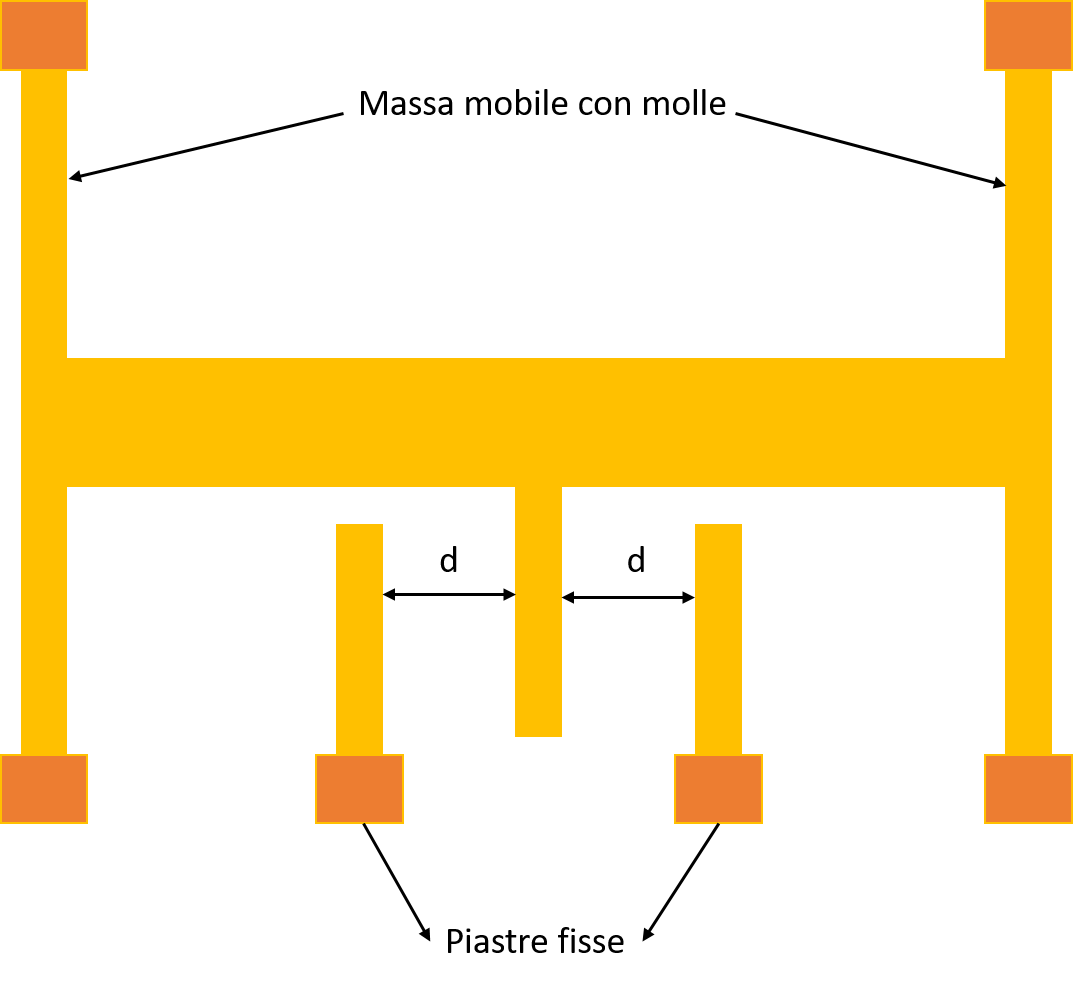
\includegraphics[scale=0.25 ]{tecnologie/acc1.png}
	\caption{Rappresentazione esemplificativa di un accelerometro capacitivo a riposo}
	\label{fig:acc1}
\end{figure}
La massa centrale è in grado di muoversi lungo un asse orizzontale grazie a delle molle poste alle sue estremità, come rappresentato dalla figura seguente:
 \begin{figure}[H]  
	\centering 
	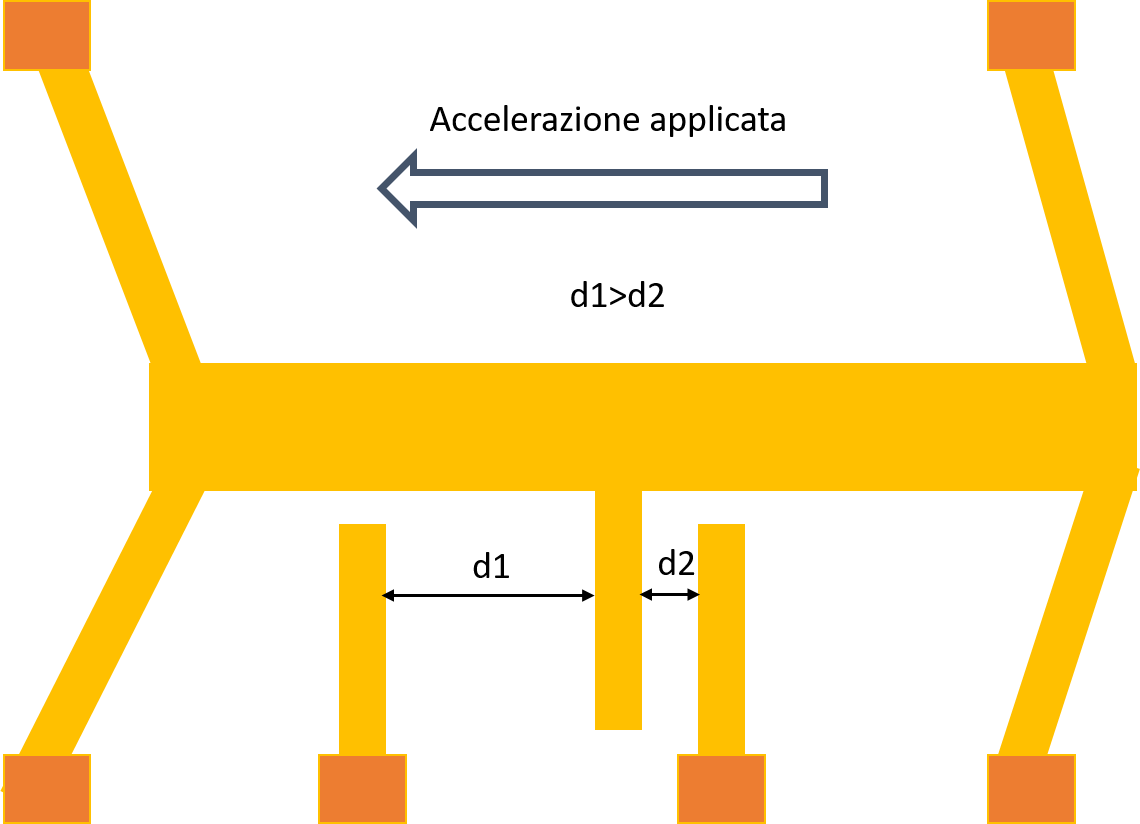
\includegraphics[scale=0.25 ]{tecnologie/acc2.png}
	\caption{Rappresentazione esemplificativa di un accelerometro capacitivo che subisce una forza esterna}
	\label{fig:acc2}
\end{figure}

A seguito del movimento della massa centrale, la distanza $d2$ in Fig.\ref{fig:acc2} si farà più piccola provocando una variazione di tensione ai capi della massa centrale. Questa verrà quindi convertita in un valore numerico rappresentante l'accelerazione subita in base alla scala e alla sensibilità del dispositivo.\\ 

\section{Giroscopio}
\label{giroscopi}
In generale, un giroscopio è un dispositivo in grado di misurare la velocità angolare a cui è sottoposto il dispositivo. I giroscopi realizzati mediante tecnologia MEMS si basano sulla forza di \textit{Coriolis}. In fisica \cite{corolois}, la forza di Coriolis è una forza apparente a cui risulta soggetto un corpo quando si osserva il suo moto da un sistema di riferimento che sia in moto circolare rispetto ad un sistema di riferimento inerziale. \\
I giroscopi di questo tipo sono composti \cite{gyroMems} da una \textit{massa}, due \textit{molle} e due ammortizzatori come mostrato in Fig.\ref{fig:gyro}. Si assuma  l'asse x come l'asse di direzione (\textit{drive mode}) e l'asse y come l'asse di rilevamento(\textit{sensing mode}). Quando la massa è sottoposta ad una vibrazione armonica applicata da una forza elettrostatica, elettromagnetica o elettrotermica lo spostamento lungo l'asse x è dato da:
\begin{equation}
x(t) = A_x \cos(\omega_x t)
\end{equation}
Dove $A_x$ è l'ampiezza e $\omega_x$ è la frequenza angolare.  Una velocità angolare $\Omega_z$ in input intorno all'asse z causa un'accelerazione di Coriolis lungo l'asse y data dalla seguente equazione:
\begin{equation}
a_y= 2\Omega_z \times \frac{d_x}{d_t}= -2\Omega_z A_x \omega_x \sin(\omega_x t)
\end{equation}

La massa quindi inizierà a vibrare lungo l'asse y a causa della forza di Coriolis e la velocità angolare $\Omega_z$ può essere calcolata misurando lo spostamento lungo l'asse vibrante. \\
Quando il \textit{drive mode} e il \textit{sense mode} sono perfettamente uguali ($\omega_x = \omega_y$), l'ampiezza lungo l'asse y raggiunge il massimo mentre la larghezza di banda raggiunge il minimo. In generale, questi due parametri dovrebbero essere uguali al fine di ottimizzare la sensibilità e la larghezza di banda.
 \begin{figure}[H]  
	\centering 
	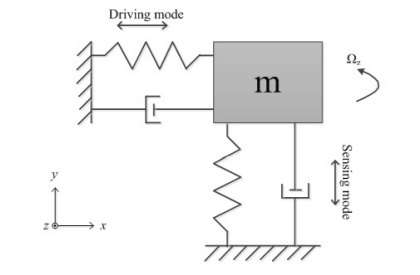
\includegraphics[scale=1]{tecnologie/gyro.png}
	\caption{Rappresentazione di un giroscopio vibrante per la misura della velocità angolare lungo l'asse z}
	\label{fig:gyro}
\end{figure}




\section{Magnetometro}
\label{magnetometro}
In generale, un magnetometro è un dispositivo in grado di rilevare l'intensità e la direzione del campo magnetico presente. Questi si basano sulla ben nota forza di Lorentz.\\
Se si eroga una certa corrente in un conduttore posto in un campo magnetico trasversale al flusso, si genera una forza proporzionale alla velocità dei portatori, alla carica ed al valore del campo magnetico, diretta nella direzione ortogonale ad entrambi, secondo la  relazione:
\begin{equation}
\overrightarrow{F_L} = q \overrightarrow{v} \times \overrightarrow{B}
\end{equation}
Dove:
\begin{itemize}
	\item $q$ è la carica elementare
	\item $F$ è la forza di Lorentz
	\item $B$ è il campo magnetico nel vuoto
\end{itemize}
Indicando con $l$ la lunghezza del conduttore si ha:
\begin{equation}
\overrightarrow{F_L} = l \overrightarrow{i} \times \overrightarrow{B}
\end{equation}
Questa forza viene quindi sfruttata per misurare il campo magnetico esterno agente sul dispositivo. Una delle realizzazioni più comuni nell'ambito dei sensori realizzati mediante tecnologia MEMS sono i magnetometri capacitivi.\\
In Fig.\ref{fig:magnet} è mostrata una semplice implementazione di un magnetometro capacitivo. Questo è composto da due \textit{molle} i cui terminali sono ancorati al substrato del dispositivo dove viene fatta circolare una corrente elettrica. Nel punto centrale le molle mantengono sospeso un \textit{rotore} dove idealmente non scorre corrente e al cui interno sono ancorati degli \textit{statori}. In presenza di una forza di Lorentz, le \textit{molle} si deformano dando origine ad uno spostamento rigido del \textit{rotore}. Poiché lo \textit{statore} non si muove, la capacità tra il \textit{rotore} e lo \textit{statore} cambia in maniera proporzionale all'intensità del campo magnetico esterno.
 \begin{figure}[H]  
	\centering 
	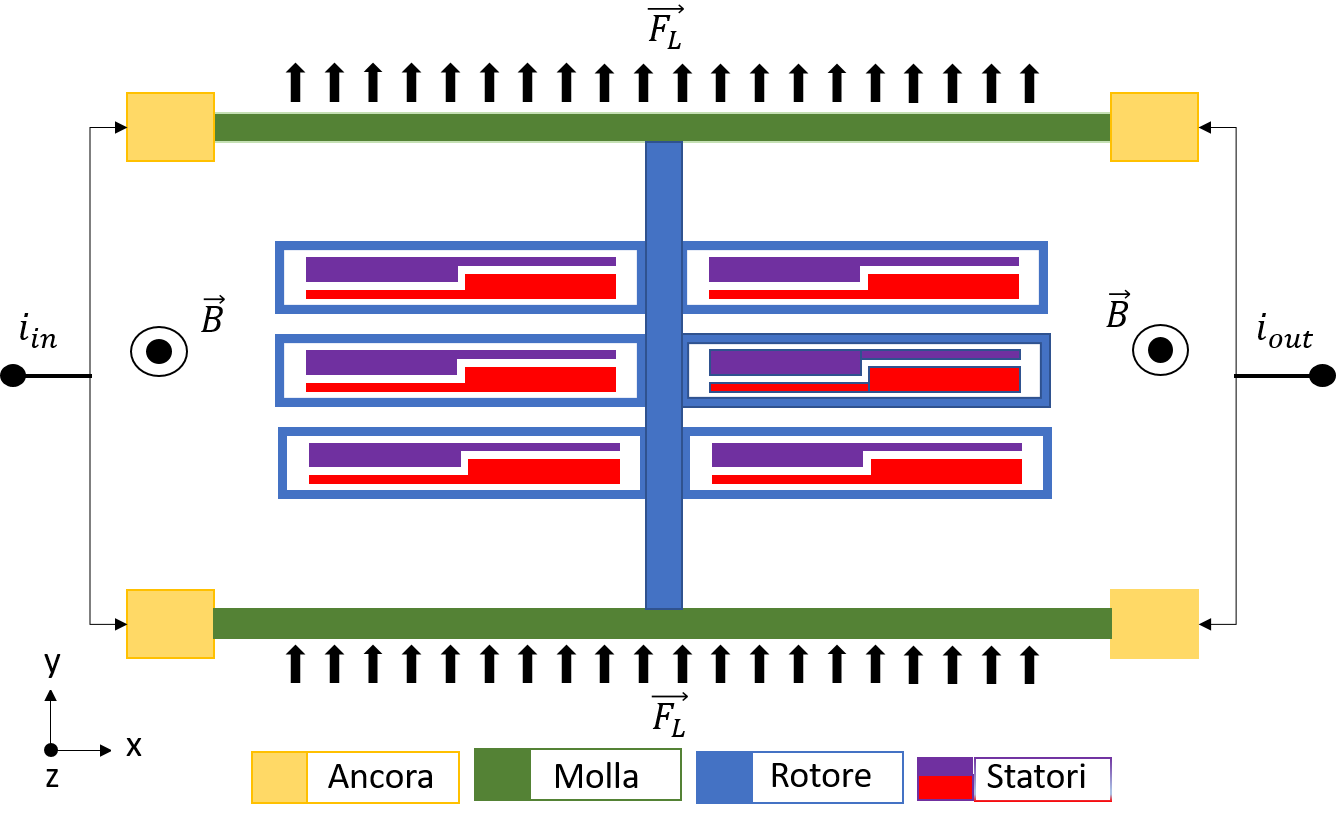
\includegraphics[scale=0.4 ]{tecnologie/magnet.png}
	\caption{Rappresentazione esemplificativa di un magnetometro capacitivo lungo l'asse \textit{z}}
	\label{fig:magnet}
\end{figure}


\section{Modello di misura}
\label{modello_di_misura}
Dopo aver introdotto i principi di funzionamento dei sensori è bene specificare il modello di misurazione.\\
I sensori utilizzati hanno tre assi lungo i quali una \textit{"quantità fisica"} (esempio forza, velocità angolare, campo magnetico) è convertita in un segnale di tensione in uscita. \\
Tipicamente questi sensori hanno un comportamento lineare nell'area di lavoro. Sulla base di questa osservazione, la seguente equazione (semplificata) descrive la relazione tra la forza fisica $y(t)$ e la tensione in uscita dal sensore $ u(t)$:

\begin{equation}
    u(t) = G R y(t) + c
\end{equation}
Dove:
\begin{itemize}
	\item $G$ è la matrice diagonale contenente il guadagno per ogni asse sensibile
	\item $R$ è la matrice di allineamento che specifica la direzione degli assi
	\item $c$ è il vettore di offset 
\end{itemize}
Al fine di discutere il modello di misura, si devono introdurre i seguenti sistemi di coordinate (in inglese: \textit{coordinate frames}) rappresentati in Fig.\ref{fig:frames}:

\begin{itemize}
	\item Il \textbf{frame del corpo} - \textit{b-frame} (in inglese: \textit{body frame}): è il sistema							 di riferimento dei movimenti dell'IMU. L'origine è posta al centro dei sensori e allineata al case posto sul chip. Tutte le misure inerziali sono calcolate su questo sistema di riferimento.
	\item Il \textbf{frame di navigazione} - \textit{n-frame} (in inglese: \textit{navigation frame}) è il frame geografico nel quale vogliamo navigare. Per navigazioni a corto raggio è considerato statico rispetto alla terra.
	\item Il \textbf{frame inerziale} - \textit{i-frame} (in inglese: \textit{inertial frame}): è un frame stazionario non rotante. L'IMU misura le forze relativamente a questo frame. La sua origine è posta al centro della terra e i suoi assi sono allineati rispetto alle stelle.
	\item Il \textbf{frame terrestre} - \textit{e-frame} (in inglese: \textit{earth frame}): coincide con l' i-frame ma ruota intorno alla terra. L'origine è posta al centro della terra e gli assi fissati rispetto ad essa.
\end{itemize}



\begin{figure}[H]
	\centering    
	\label{fig:frames}
	\subfigure[]{\label{fig:framesa}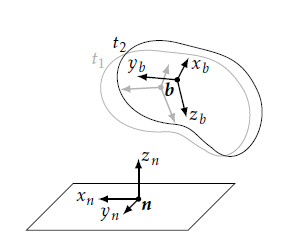
\includegraphics[width=60mm]{tecnologie/framesa.png}}
	\subfigure[]{\label{fig:framesb}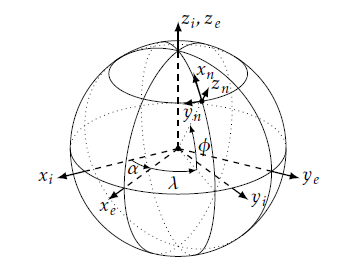
\includegraphics[width=60mm]{tecnologie/framesb.png}}
	\caption{in \ref{fig:framesa} il \textit{b-frame} nell'istante $t_1$ e $t_2$ relativamente al \textit{n-frame}, in \ref{fig:framesb} l'\textit{n-frame} in latitudine $\varphi$ e longitudine $\lambda$, l'\textit{e-frame} all'angolo $\alpha(t)= \omega_{ie}t$ e l'\textit{i-frame}}
\end{figure}
Ignorando la dipendenza dal tempo delle quantità coinvolte, la misura del giroscopio (si veda \ref{giroscopi}) è modellata in \cite{gyromodel} come:

\begin{equation}
y_\omega = \omega_{ib}^b + \delta_{\omega}^b + e_\omega^b
\end{equation}

Dove:
\begin{itemize}
	\item $\omega_{ib}$ è la velocità angolare nel \textit{b-frame} osservata dall'\textit{i-frame}
	\item $\delta_\omega$ è la deriva del sensore che varia lentamente nel tempo 
	\item $e_w^b$ è il rumore gaussiano
\end{itemize}

La velocità angolare $\omega_{ib}$ può essere così estesa:

\begin{equation}
\omega_{ib} = R^{bn} ( \omega_{ie}^n + \omega_{en}^n) + \omega_{nb}^b
\end{equation}

Dove:
\begin{itemize}
	\item $ R$ è la matrice di rotazione
	\item $\omega_{ie}$ è la velocità angolare della terra
	\item $\omega_{en}$ è velocità angolare di transporto
	\item $\omega_{nb}$ è la velocità angolare richiesta ai fini della navigazione
\end{itemize}

La misura dell'accelerometro $y_a$ è invece modellata in \cite{gyromodel} come:

\begin{equation}
\label{accelModel}
 y_a = f^b + \delta_a^b + e_a^b = R^{bn} (\ddot{b}_{ii}^n - g^n) + \delta_a^b + e_a^b
\end{equation}
Dove:
\begin{itemize}
	\item $f$ è la specifica forza esterna
	\item $\delta_a$ è la deriva del sensore che varia lentamente nel tempo 
	\item $e_a$ è il rumore gaussiano
\end{itemize}
L'Eq.\ref{accelModel} divide la forza specifica nei suoi contributi provenienti dall'accelerazione lineare del corpo osservata dall'\textit{i-frame} ($\ddot{b}_{ii}$) e dal vettore gravitazione $g$. L'accelerazione lineare può a sua volta essere espansa come:

\begin{equation}
\ddot{b}_{ii} = \omega_{ie}^n \times \omega_{ie}^n \times R^{ni}b^i + 2\omega_{ie}^n \times \dot{b_n^n}+\ddot{b_{nn}^n}
\end{equation}

dove $\ddot{b_{nn}}$ è l'accelerazione del corpo osservata dal \textit{n-frame} richiesto per la navigazione.\\

Infine per il magnetometro (si veda \ref{magnetometro}) la misura $y_m$ è così modellata:

\begin{equation}
y_m = m^b + e_b^b = R^{bn} m^n + e_m^b
\end{equation}
Dove:
\begin{itemize}
	\item $m$ è il vettore del campo magnetico locale
	\item $e_m$ è il rumore gaussiano
\end{itemize}
In assenza di oggetti ferromagnetici, $m$ è il campo magnetico della terra e la misura del magnetometro può essere usata come una bussola per trovare la direzione del nord magnetico.







